\chapter{Conclusion}\label{conclusion}

\section{Science-Driven Technological Development}

The ambitious science goals of current and next generation sub-mm/mm-wave observatories drives the development of new technologies at a rapid pace. Upcoming ground-based observatories which will probe the inflationary epoch through measurements of B-mode polarization in the CMB (e.g., Simons Observatory \citep{ade2019simons}, AliCPT \citep{li2018probing}, CMB-S4 \citep{abitbol2017cmb}) require detector multiplexing factors of $\mathcal{O}(10^{5}--10^{6})$. These multiplexing factors exceed the capabilities of preexisting DSP boards, such as the CASPER ROACH2, by an order of magnitude.

From a SWAP-C standpoint, the need for higher multiplexing factors cannot be met by simply scaling up current systems. The current per-pixel cost of MKID readout systems with multiplexing factors of $\sim$1000 (e.g., BLAST-TNG, TolTEC and DARKNESS) is $\sim$1~USD/pixel. Additionally, the increase in size, weight and power dissipation of the scaled-up systems would impose thermal and mass budgets which prohibit their use on planned space-based sub-mm/FIR surveyors (e.g., LiteBIRD \citep{matsumura2014mission}, Origins Space Telescope \citep{battersby2018origins}).

The solutions to the limitations inherent in current systems will incorporate novel electronics and DSP algorithms developed by scientific collaborations, as well as new technologies which are emerging from the commercial sector. The scaling down of hardware and electronics includes both the digital and analog (IF/RF) sets of electronics. This process has already begun for the systems which will be used by upcoming sub-mm balloon experiments (e.g., EXCLAIM and TIM).

Figure~\ref{fig:toltec slice} shows one of the TolTEC IF electronics slices, which was assembled at ASU. It is based on the BLAST-TNG IF electronics, combining COTS components, such as the modulator and demodulator, with custom components designed at ASU, such as the anti-aliasing filters and programmable attenuators. Figure~\ref{fig:single board} shows an equivalent system (also designed at ASU) which has been scaled down to a single multi-layer PCB which is many times smaller than the baseline IF system. Single-board systems like this offer significant SWAP-C advantages.

The SWAP-C of the digital electronics is also undergoing rapid improvements. One example of this is the Xilinx RF System on a Chip\footnote{\url{https://www.xilinx.com}} (RFSoC) family of integrated RF-FPGA systems. The RFSoC, which is based on the Zynq UltraScale+ FPGA, incorporates up to 16 14-bit DACs and 16 12-bit ADCs on a single chip, and has an instantaneous RF bandwidth of several gigahertz. The expanded signal bandwidth is accompanied by SWAP-C improvements of several orders of magnitude, which directly translate into lower cost-per-pixel. Efforts to port existing MKID and TES FPGA firmware designs, including the BLAST-TNG firmware, are already underway.

The larger FPGA fabric provided by these new commercial boards allows for the implementation of improved detector readout algorithms for both MKIDs and TESs which up until now have only been possible with the use of custom electronics. One example of this is the `tone-tracking' algorithm which is used by the SLAC Microresonator Radio Frequency (SMuRF) readout \citep{henderson2018highly}. SMuRF is the readout system for Simons Observatory, which uses a detector technology called microwave frequency domain multiplexing ($\mu$MUX \cite{irwin2004microwave}).

$\mu$MUX systems use TES sensors which are inductively coupled to RF SQUIDs which form part of a resonator circuit. In this way, they can be frequency domain multiplexed and readout using FDM algorithms similar to those which are used for KID readout. Tone-tracking refers to the process of making high speed changes to the amplitude and frequency of each probe tone in a multitone readout comb in order to compensate for changes in the responsivity of each pixel. The level of difficulty which is involved in implementing tone-tracking depends on the method which is used to calculate the required adjustments, as well as the method which is used to synthesize the probe tones.

In the ASU LEKID readout system, the tone comb is synthesized in software, and then stored in RAM on the ROACH2 board. One shortcoming of this method of tone synthesis is that in order to change either the frequency, amplitude or phase of a single tone in the comb, the entire comb must be resynthesized. Rewriting the tone comb to RAM takes $\sim$3~seconds, making resonator tuning a very slow process.

During the 2018 OLIMPO flight, it took $\sim$1~hr to tune 120 pixels \citep{masi2019kinetic}. Using the CORDIC algorithm (COordinate Rotation DIgital Computer) for tone synthesis, the parameters of each probe tone can be tweaked independently of all of the others, at a very high rate. This opens up the possibility of trying many different tone-tracking algorithms, which are not possible to implement on a ROACH2 system due to the limited size of the FPGA fabric.

\begin{figure}[!htbp]
\centering
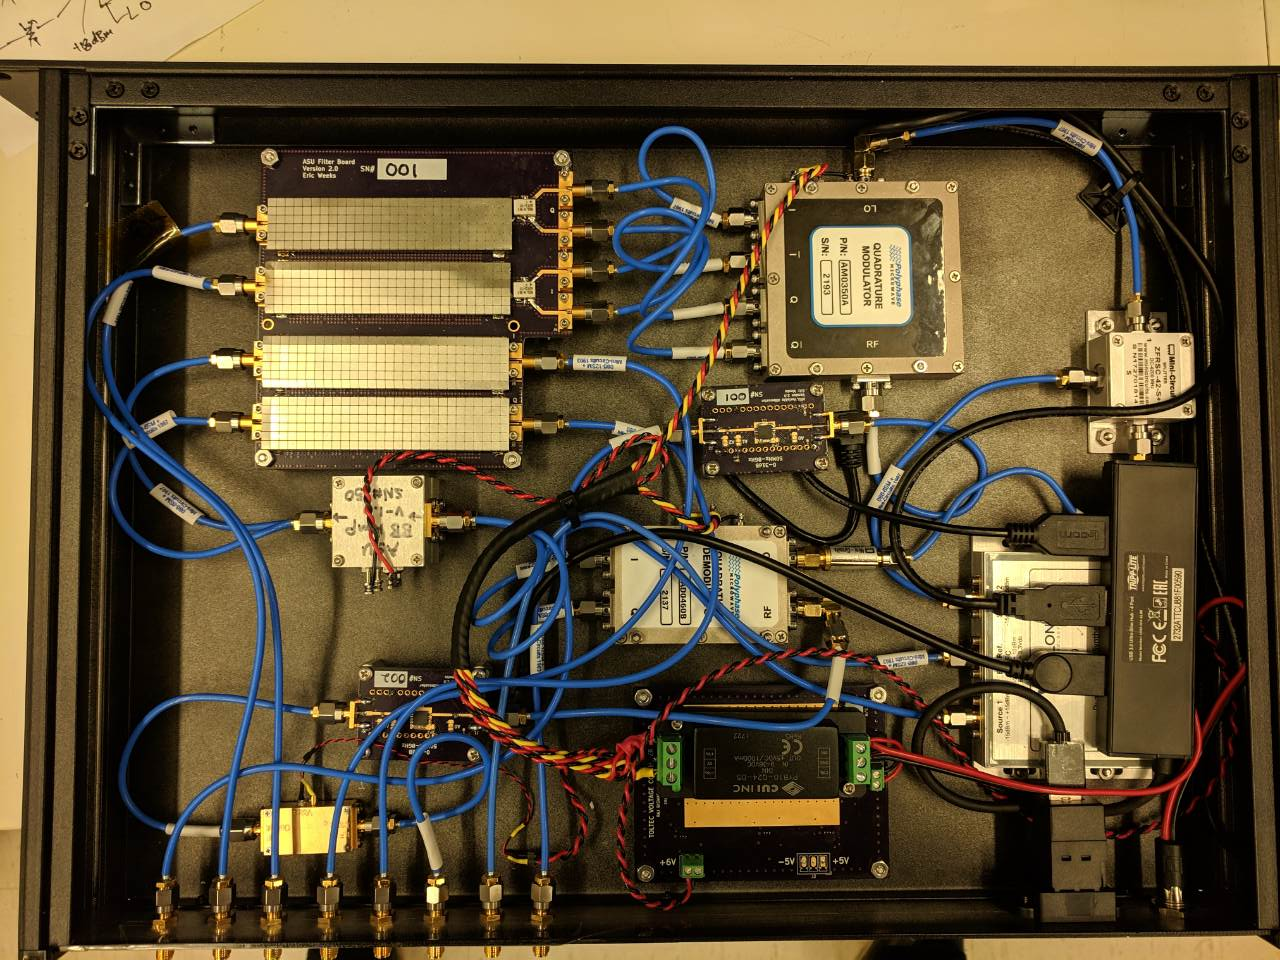
\includegraphics[width=\textwidth]{figures/conclusion/toltec_slice_2}
\caption[~An IF electronics slice for TolTEC.]{An IF electronics slice for TolTEC.}
\label{fig:toltec slice}
\end{figure}

\begin{figure}[!htbp]
\centering
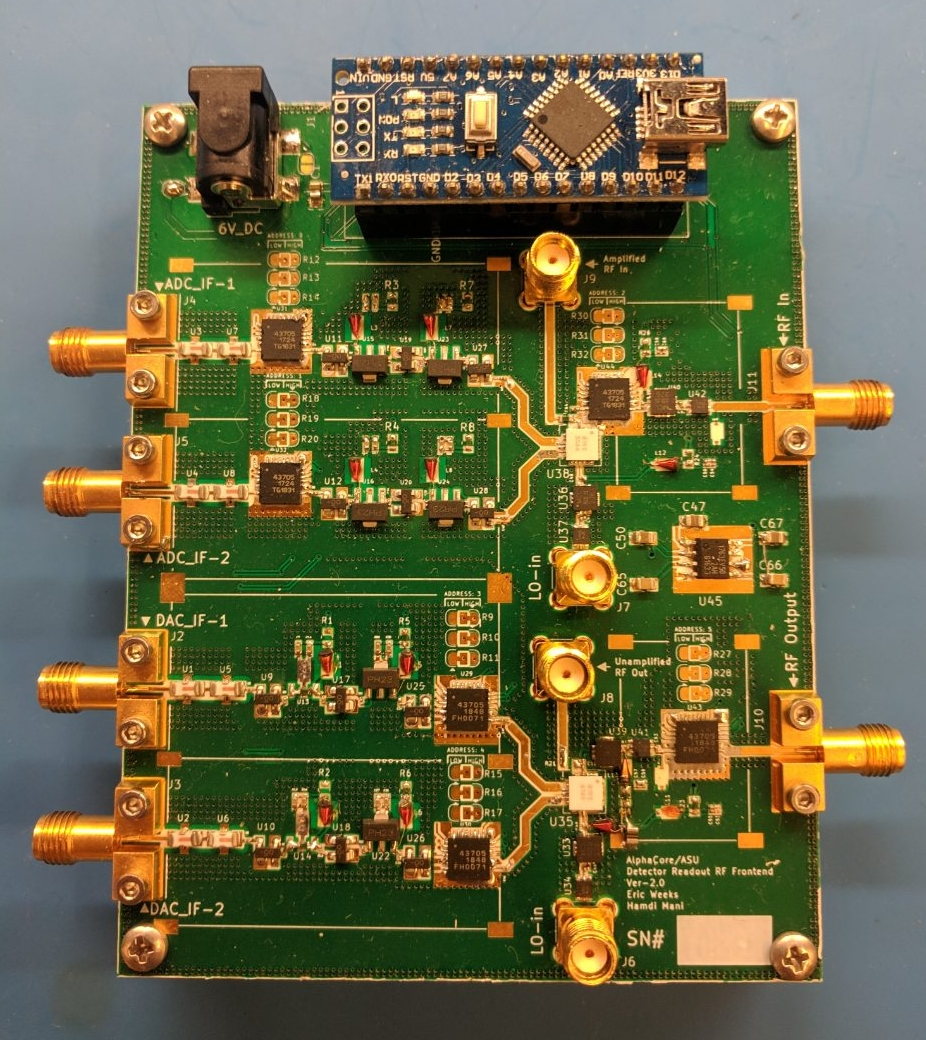
\includegraphics[width=0.7\textwidth]{figures/conclusion/single_board}
\caption[~A single-board board implementation of the TolTEC IF electronics.]{A single-board board implementation of the TolTEC IF electronics. Image credit: Eric Weeks.}
\label{fig:single board}
\end{figure}
